\subsection{Transmission Control Protocol}

    Si tratta di un protocollo che offre un servizio di comunicazione fra processi affidabile e con connessione.
    
    \vspace{3mm}
    
    Poiché il processo mittente e il processo destinatario potrebbero non scrivere e leggere alla stessa velocità, il protocollo TCP utilizza dei buffer per memorizzare sia il flusso di dati in uscita dla processo mittente, sia il flusso di dati in entrata per il processo destinatario.
    
    \vspace{3mm}
    
    I buffer sono code circolari di celle di memoria, ognuna capace di contenere 1 byte. 
    
    \vspace{3mm}
    
    Il \textbf{buffer del mittente} è diviso in tre zone: la \textit{zona bianca} (contenente celle di memoria utilizzate dal processo mittente per scrivere nuovi byte da spedire - quando si scrive su una zona bianca, essa diventa colorata), la \textit{zona grigia} (contenente i dati spediti ma non ancora riscontrati dal destinatario), la \textit{zona colorata} (contenete l'insieme dei dati che il mittente ha già scritto, ma che il protocollo non ha ancora inviato). Se il buffer si riempie, la trasmissione va rallentata.
    
    \vspace{3mm}
    
    Il \textbf{buffer del destinatario} è diviso in due zone: la \textit{zona bianca} (contenente celle vuote da riempire coi byte in arrivo) e la \textit{zona colorata} (contenente i byte ricevuti, ma che il processo destinatario non ha ancora accolto - quando un byte viene letto dal processo, la corrispondente cella del buffer viene riciclata).
    
    \vspace{3mm}
    
    Il flusso di dati, quindi il messaggio, prende il nome di \textbf{segmento}. Lo strato di trasporto prende il segmento e ci aggiunge una intestazione. I segmenti devono essere riassemblati e spediti in ordine al processo destinatario. TCP è affidabile proprio perché riassembla i segmenti e si assicura che ci siano tutti.
    
    L'ordine del riassemblaggio si garantisce assegnando ad ogni segmento un opportuno numero di sequenza (32 bit) che specifica il numero di sequenza del primo byte contenuto nel segmento.
    
    \vspace{3mm}
    
    La comunicazione è bidirezionale: il processo mittente deve sapere quando i dati sono arrivati a destinazione, e per ottenere questo risultato si usa il \textbf{numero di riscontro} (32 bit). 
    
    Per evitare il numero di messaggi scambiati che contengono solo i numeri di riscontro, il protocollo utilizza una tecnica detta \textbf{piggyback}: i numeri di riscontro vengono inseriti nei pacchetti dati della risposta da parte del server. Il numero di riscontro rappresenta il numero del prossimo byte che il destinatario si aspetta di ricevere, ed è cumulativo. In termini pratici, se il destinatario spedisce un numero di riscontro pari a $x$, sta dicendo di mittente di aver ricevuto fino al byte $x-1$.
    
    \vspace{3mm}
    
    TCP offre funzionalità per il controllo del flusso, degi errori e della congestione, come definito in precedenza. 
    
    In caso di errori, i segmenti vengono rispediti.
    
    \subsubsection{Formato TCP}
    
        L'intestazione del segmento (e non datagram!) TCP ha una lunghezza minima di 20 byte e un massima di 60 byte.
        
        \begin{itemize}
            \item 
                \textbf{Porta sorgente (16 bit).} Specifica il numero di porta utilizzato dal processo mittente.
                
            \item 
                \textbf{Porta mittente (16 bit).} Specifica il numero di porta utilizzato dal processo destinatario.
                
            \item 
                \textbf{Numeri di riscontro (32 bit).} Rappresenta il numero di sequenza del primo byte contenuto nella sezione dati del segmento.
                
            \item 
                \textbf{Numeri di riscontro (32 bit).} Specifica il numero del prossimo byte che il destinatario si aspetta di ricevere dal mittente. Il numero di riscontro è valido solo quando il bit di controllo ACK vale 1.
                
            \item 
                \textbf{Lunghezza intestazione (4 bit).} Misurato in gruppi da 4 byte. Rappresenta la lunghezza dell'intero segmento.
                
            \item 
                \textbf{Bit riservati (6 bit).} Riservato ad utilizzi futuri.
                
            \item 
                \textbf{Bit di controllo.} Utilizzati per vari scopi. Sono attivati con un opportuno flag 0/1.
                    \begin{itemize}
                        \item 
                            \textbf{URG.} Puntatore dati urgente.
                        
                        \item 
                            \textbf{ACK.} Bit di riscontro.
                            
                        \item 
                            \textbf{PSH.} Richiesta di spedizione immediata.
                            
                        \item 
                            \textbf{RST.} Interrompi la connessione.
                            
                        \item 
                            \textbf{SYN.} Instaura la connessione.
                            
                        \item 
                            \textbf{FIN.} Chiudi la connessione.
                    \end{itemize}
                    
            \item 
                \textbf{Lunghezza della finestra (fino a 65535 byte).} Il nodo destinatario, all'interno di questo campo, specifica il numero massimo di byte che è in grado di supportare. Permette di garantire il controllo del flusso.
                
            \item
                \textbf{Somma di controllo.} Come per UDP.
                
            \item
                \textbf{Puntatore dati urgenti.} Valido se il flag di URG è 1. Indica che il segmento sta trasportando dati urgenti (cioè dati che sostano per un brevissimo perido sul buffer - si tratta di un diritto di prelazione). Indica, in particolare, la fine dei dati urgenti (in termini di byte).
                
            \item
                \textbf{Opzioni (fino a 40 byte).}
        \end{itemize}
        
    \subsubsection{Three-Way-Handshaking}
    
        Mittente e destinatario devono creare una sorta di collegamento virtuale, e questo processo richiede tre fasi, realizzate tramite il protocollo Three-Way-Handshaking: instaurazione della connessione, trasferimento dati e chiusura della connessione. Tale collegamento facilita l'implementazione delle caratteristiche offerte dal TCP. 
        
        \subsubsubsection{Apertura della connessione}
        
            Un processo locale sul client vuole iniziare una comunicazione con un processo remoto sul server. Il processo locale esegue un'\textit{apertura attiva}, e il server risponde con un'\textit{apertura passiva} (mettendosi in attesa in eventuali richieste).
                
            \vspace{3mm}
                
            A questo punto, il client intende instaurare una connessione col server: intuitivamente, vengono spediti tre messaggi che contegono informazioni su "come mettersi d'accordo" per i spedire i messaggi effettivi. Li si pensi come a dei "meta-messaggi".
                
            \vspace{3mm}
                
            Far partire l'apertura attiva significa proprio mandare uno di questi messaggi, detto segmento di sincronizzazione (col bit di controllo SYN a 1). Questo segmento è funzionale alla sincronizzazione dei numeri di sequenza: il numero di sequenza specificato nel segmento viene scelto in modo casuale dal client, e rappresneta l'inizio della numerazione dei dati del messaggio da spedire alla fine dell'handshake.
                
            \vspace{3mm}
                
            Il server risponde con un segmento, detto di SYN+ACK (e quindi con queste due flag ad 1), che ha un numero di sequenza differente dal precedente, e che ha la doppia funzione di assicurare la bidirezionalità della comunicazione, e di riscontrare la ricezione del primo segmento. Il valore del bit di ACK è il numero di sequenza + 1. Se il numero di sequenza del primo segmento era 8000, il bit di ACK varrà 8001. Il segmento contiene anche la dimensione della finestra (e cioè "quanti dati" sono disposta a ricevere, inteso come la dimensione massima del segmento).
                
            \vspace{3mm}
                
            L'ultimo segmento è spedito dal client ed è fondamentalmente un riscontro del precedente segmento. Contiene solo l'ACK (numero di sequenza del precedente segmento + 1).
                
            \vspace{3mm}
                
            Il giro quindi è SYN - SYN+ACK - ACK. Al termine dell'ultima spedizione, la connessione è stabilita e aperta, e si può procedere al trasferimento dei dati utilizzando il piggyback.
            
        \subsubsubsection{Trasferimento dati}
        
            L'unica aggiunta da fare a ciò che è stato già detto è che i segmenti dati spediti dal client viaggiano con il bit di controllo PSH impostato a 1. Questo bit segnala al TCP di consegnare i dati al processo server appena essi vengono ricevuti.
            
            Il vantaggio dell'uso del bit PSH è che aumenta l'efficienza. Lo svantaggio è che può provocare dei ritardi sia nella spedizione che nella consegna dovuti al passaggio dei dati nei buffer.
            
        \subsubsubsection{Chiusura della connessione}
        
            La chiusura può essere di due tipi: three-way o four-way.
            
            \vspace{3mm}
            
            \textbf{Chiusura Three-Way}
            
                \vspace{3mm}
            
                Il client vuole chiudere la connessione, e manda un segmento con bit di controllo FIN a 1.
                
                Il server riceve il segmento e risponde con un segmento dotato di FIN+ACK (che rispetta sempre la quantificazione illustrata in precedenza); il client riceve la risposta e risponde a sua volta con un altro ACK. Il giro è FIN - FIN+ACK - ACK.
                
                \vspace{3mm}
                
            \textbf{Chiusura Four-Way}
            
                \vspace{3mm}
            
                Se il server ha ancora dei dati da spedire, si usa questa tecnica.
                
                Il client spedisce un FIN, il server risonde con ACK. Tuttavia, il server ha ancora dei dati da spedire, quindi dopo il trasferimento spedisce un FIN al client, il quale risponderà con un ACK. Il giro è FIN - ACK [..] FIN - ACK.
                
                Questa tecnica definisce il "caso peggiore" dei segmenti necessari ad aprire e chiudere una connessione, cioè 7. In generale, gli $n$ pacchetti necessari alla gestione della connessione sono detti di \textit{overhead}.
                
    \begin{center}
        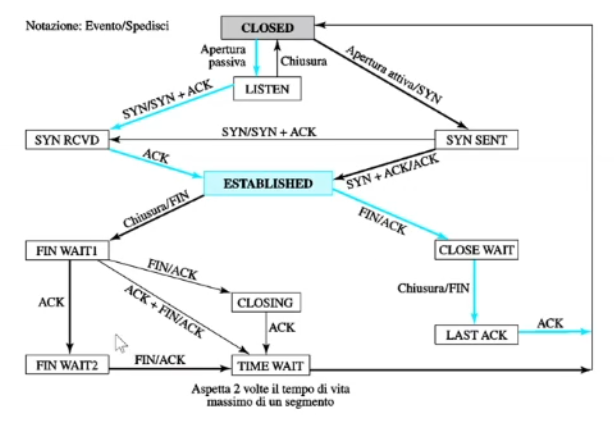
\includegraphics[scale=0.5]{images/Diagramma-di-Stato.png}
    \end{center}
    
    \subsubsection{Finestre di scorrimento e Algoritmo di Nagle}
    
        Usa un meccanismo simile a Go-Back-N dello strato di collegamento.
        
        Il destinatario accetta dati che arrivano fuori ordine e li mantiene aspettando che arrivino quelli mancanti.
        
        La differenza fra l'utilizzo della finestra scorrevole dello strato di collegamento e quella del TCP è che in quest'ultima la dimensione è variabile e ha come elementi i byte, mentre la prima aveva una dimensione fissa e impiegava i frame.
        
        La finestra scorrevole del TCP ha due limiti, uno destro e uno sinistro. La finestra può essere aperta, facendo avanzare il limite destro e permettere la spedizione di nuovi byte, e chiusa.
        
        La dimensione della finestra viene determinata dal minimo fra le dimensioni della fienstra del recivitore e la finestra di congestione. La prima è il valore che viene comunicato dal destinatario nell'instaurazione della connessione, la seconda è un valore determinato dalla capacità della rete. Il destinatario può dunque far diventare 0 la dimensione della finestra per non permettere al mittente di spedire altri dati.
        
        \vspace{3mm}
        
        Se la finestra è molto piccola, si creano segmenti che contengono pochi dati e pertanto si crea molto sovraccarico dovuto alle intestazioni. Questo problema è conosciuto come \textbf{finestra futile}, e la soluzione è imporre una limitazione a TCP, che consiste nel spedire dati solo quando la finestra è sufficientemente grande. Una soluzione alternativa è l'attesa di un certo intervallo di tempo. Una soluzione ancora più elegante è l'\textbf{algoritmo di Nagle}.
        
        \vspace{3mm}
        
        L'algoritmo di Nagle prevede di creare segmenti grandi quando possibile; se invece si trattano segmenti piccoli, allora si spedisce solo se ci sono dati riscontrati. Non so di preciso cosa significhi.
        
    \subsubsection{Controllo degli errori}
    
        I meccanismi di controllo degli errori nel TCP sono i seguenti.
        
        \begin{itemize}
            \item 
                \textbf{Somma di controllo.} Ogni segmento TCP include un campo di 16 bit per la somma di controllo, che viene utilizzato per verificare l'integrità dei dati. Se il segmento è alterato, esso viene eliminato ed è considerato come 'mai arrivato'.
            \item
                \textbf{Riscontri.} Il TCP usa i numeri di riscontri per confermare la ricezione dei segmenti. Se non ci sono dati da spedire nella direzione opposta, TCP spedisce un segmento contenente solo il numero di riscontro.
                
            \item
                \textbf{Ritrasmissione.} Una volta rilevato l'errore, bisogna correggerlo. La tecnica utilizza dal TCP riguarda la ritrasmissioine in toto dei dati. Può avvenire alla scadenza di un timout o quando vengono ricevuti tre riscontri uguali. 
            
            \item
               \textbf{Segmenti fuori ordine.} Quando un segmento viene ritardato, perduto o eliminato, i segmenti che lo seguono arrivano fuori ordine. La maggior parte delle attuali implementazioni del TCP non elimina i segmenti fuori ordine, ma li memorizza temporaneamente nella speranza che il segmento mancante arrivi. 
        \end{itemize}
        
    \subsubsection{Controllo della congestione}
    
        